%%%%%%%%%%%%%%%%%%%%%%%%%%% Julien %%%%%%%%%%%%%%%%%%%%%%%%%%%%%
\section{Parameters}

%- 1 -%
\begin{frame}{Model Parameters}{List of Parameters}
  \begin{table}[H]\centering
  \begin{tabular}{|c|S[table-figures-exponent=1]@{\,}|s[table-unit-alignment = left]|}
    \hline
      \textbf{Parameter}  & \multicolumn{1}{c|}{\textbf{Value}} & \multicolumn{1}{c|}{\textbf{Unit}}\\
    \hline%------------------------------------------------------------------
      \si{m_W}            & 0.222                               & \kilo\gram\\
    % \hline%------------------------------------------------------------------
      \si{l_W}            & 0.093                               & \metre\\
    % \hline%------------------------------------------------------------------
      \si{J_W}            & 0.601e-3                            & \kilo\gram\meter\squared\\
    % \hline%------------------------------------------------------------------
      \si{B_W}            & 17.03e-6                            & \newton\metre\second\per\radian\\
    % \hline%------------------------------------------------------------------
      \si{m_F}            & \multicolumn{1}{c|}{?}              & -\\
    % \hline%------------------------------------------------------------------
      \si{l_F}            & \multicolumn{1}{c|}{?}              & -\\
    % \hline%------------------------------------------------------------------
      \si{J_F}            & \multicolumn{1}{c|}{?}              & -\\
    % \hline%------------------------------------------------------------------
      \si{B_F}            & \multicolumn{1}{c|}{?}              & -\\
    \hline%------------------------------------------------------------------
  \end{tabular}
  \end{table}
\end{frame}

%- 2 -%
\subsection{Model Parameters}
\begin{frame}{Model Parameters}{Obtaining New Parameters}
  \begin{itemize}
    \item Mass of the frame
  \end{itemize}
  \only<2>{
    \begin{figure}[H]
      \centering
      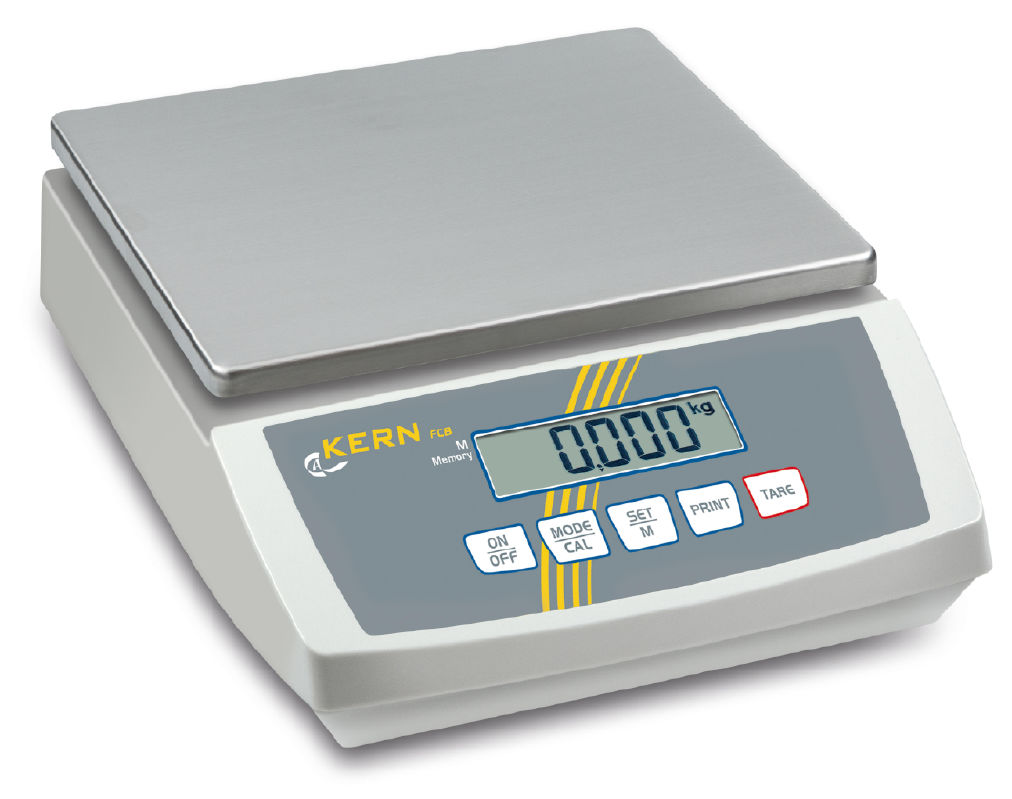
\includegraphics[scale=0.2]{Pictures/scale.jpg}
    \end{figure}
  }
  %%
  \begin{itemize}
    \item Center of mass
  \end{itemize}
  \only<3>{
  \begin{figure}[H]
    \centering
    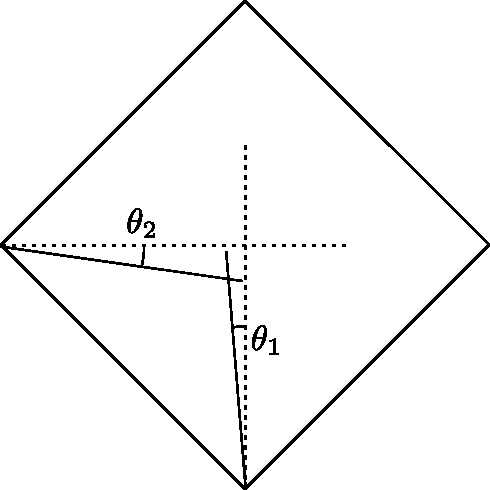
\includegraphics[scale=0.35]{Pictures/centerOfMassDiagram.pdf}
  \end{figure}
  }
  %%
  \begin{itemize}
    \item Friction and moment of inertia of the frame
  \end{itemize}
  \only<4>{
    \begin{figure}[H]
    \centering
    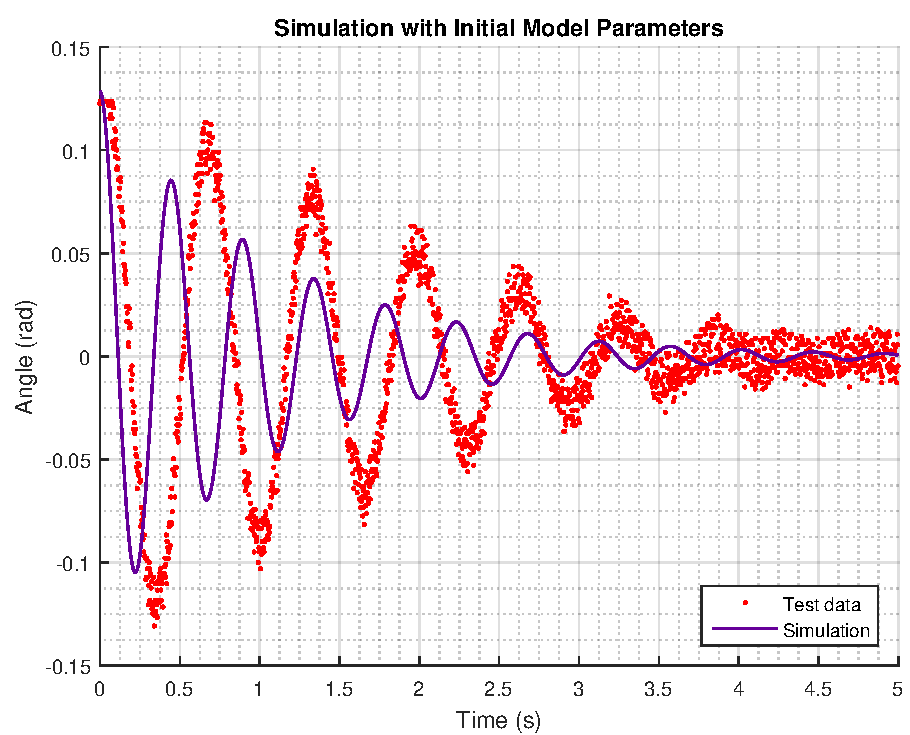
\includegraphics[scale=0.35]{Pictures/InitialModelParameterCompare.pdf}
  \end{figure}
  }
\end{frame}

%--------------------------------------------------------
\subsection{Parameter Estimation}

%- 3 -%
\begin{frame}{Parameter Estimation}{Optimization Problem}
  \begin{itemize}
    \item Optimization problem
  \end{itemize}  
  \begin{figure}[H]
      \centering
      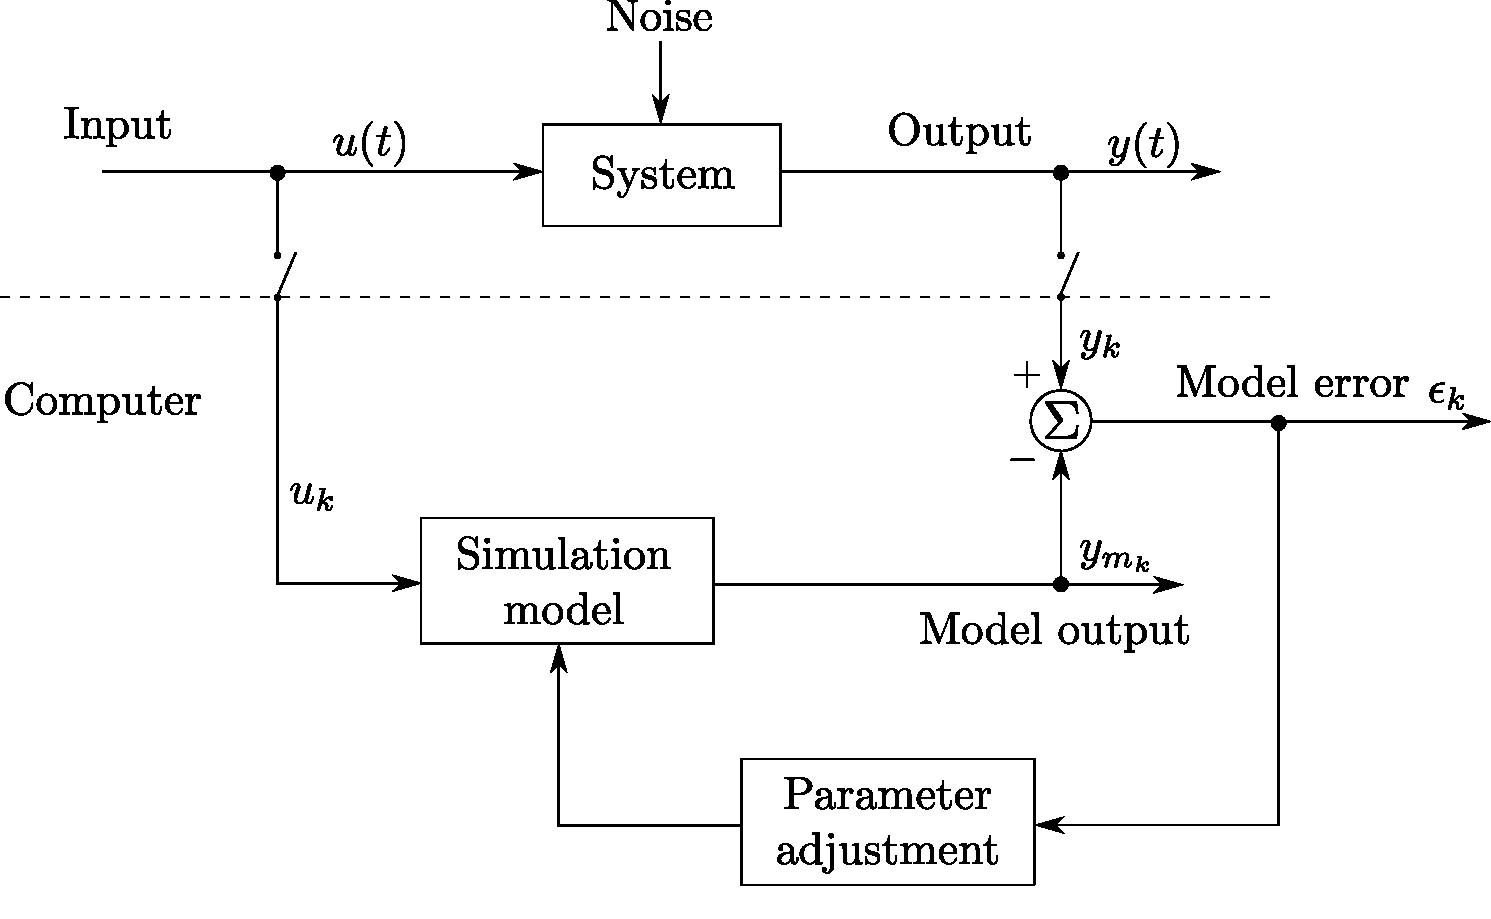
\includegraphics[scale=0.25]{Pictures/senstoolsModelOptimizationHM}
  \end{figure}\vspace{-12pt}
  \pause
  \begin{itemize}
    \item Cost function
  \end{itemize}
  \begin{displaymath}
    \si{C(\theta) = \frac{1}{2N}\sum_{k = 1}^{N} \left(y_{k} - y_{m_k}(\vec{\theta})\right)^2 }
  \end{displaymath}
\end{frame}

%- 4 -%
\begin{frame}{Parameter Estimation}{Steepest Descent}
  \begin{itemize}
    \item Taylor series expansion (2\si{^{nd}} order)
  \end{itemize}
  \begin{displaymath}
    \si{f(\vec{x}+\vec{\delta}) \approx f(\vec{x}) + \vec{g}^T \vec{\delta} + \frac{1}{2} \vec{\delta}^T \vec{H}\vec{\delta}}
  \end{displaymath}
  \begin{displaymath}
    \vdots
  \end{displaymath}
  \begin{displaymath}
    \si{\nabla\ f(\vec{x}+\vec{\delta}) \approx \vec{g}}
  \end{displaymath}
  \vspace{-12pt}
  %%
  \pause
  \begin{itemize}
    \item Reducing the problem
  \end{itemize}
    \begin{minipage}{\linewidth}
    \begin{minipage}{0.35\linewidth}
      \begin{figure}[H]
        \centering
        Arbitrary 2D cost function with the gradient direction at one starting point
        % 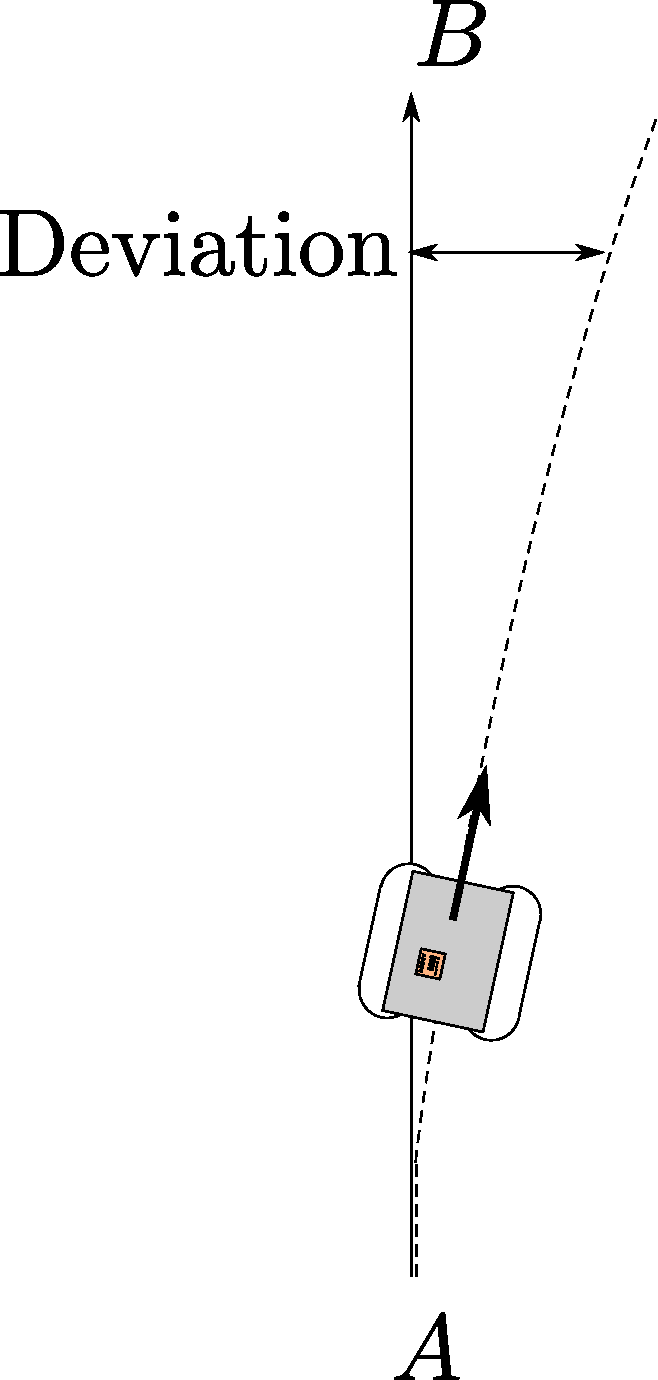
\includegraphics[scale=0.25]{Pictures/vehicleLineDeviation.pdf}
      \end{figure}
    \end{minipage}
    \hspace{0.03\linewidth}
    \begin{minipage}{0.45\linewidth}
      \begin{figure}[H]
        \centering
        Plot of the 1D cost function along the gradient direction
        % 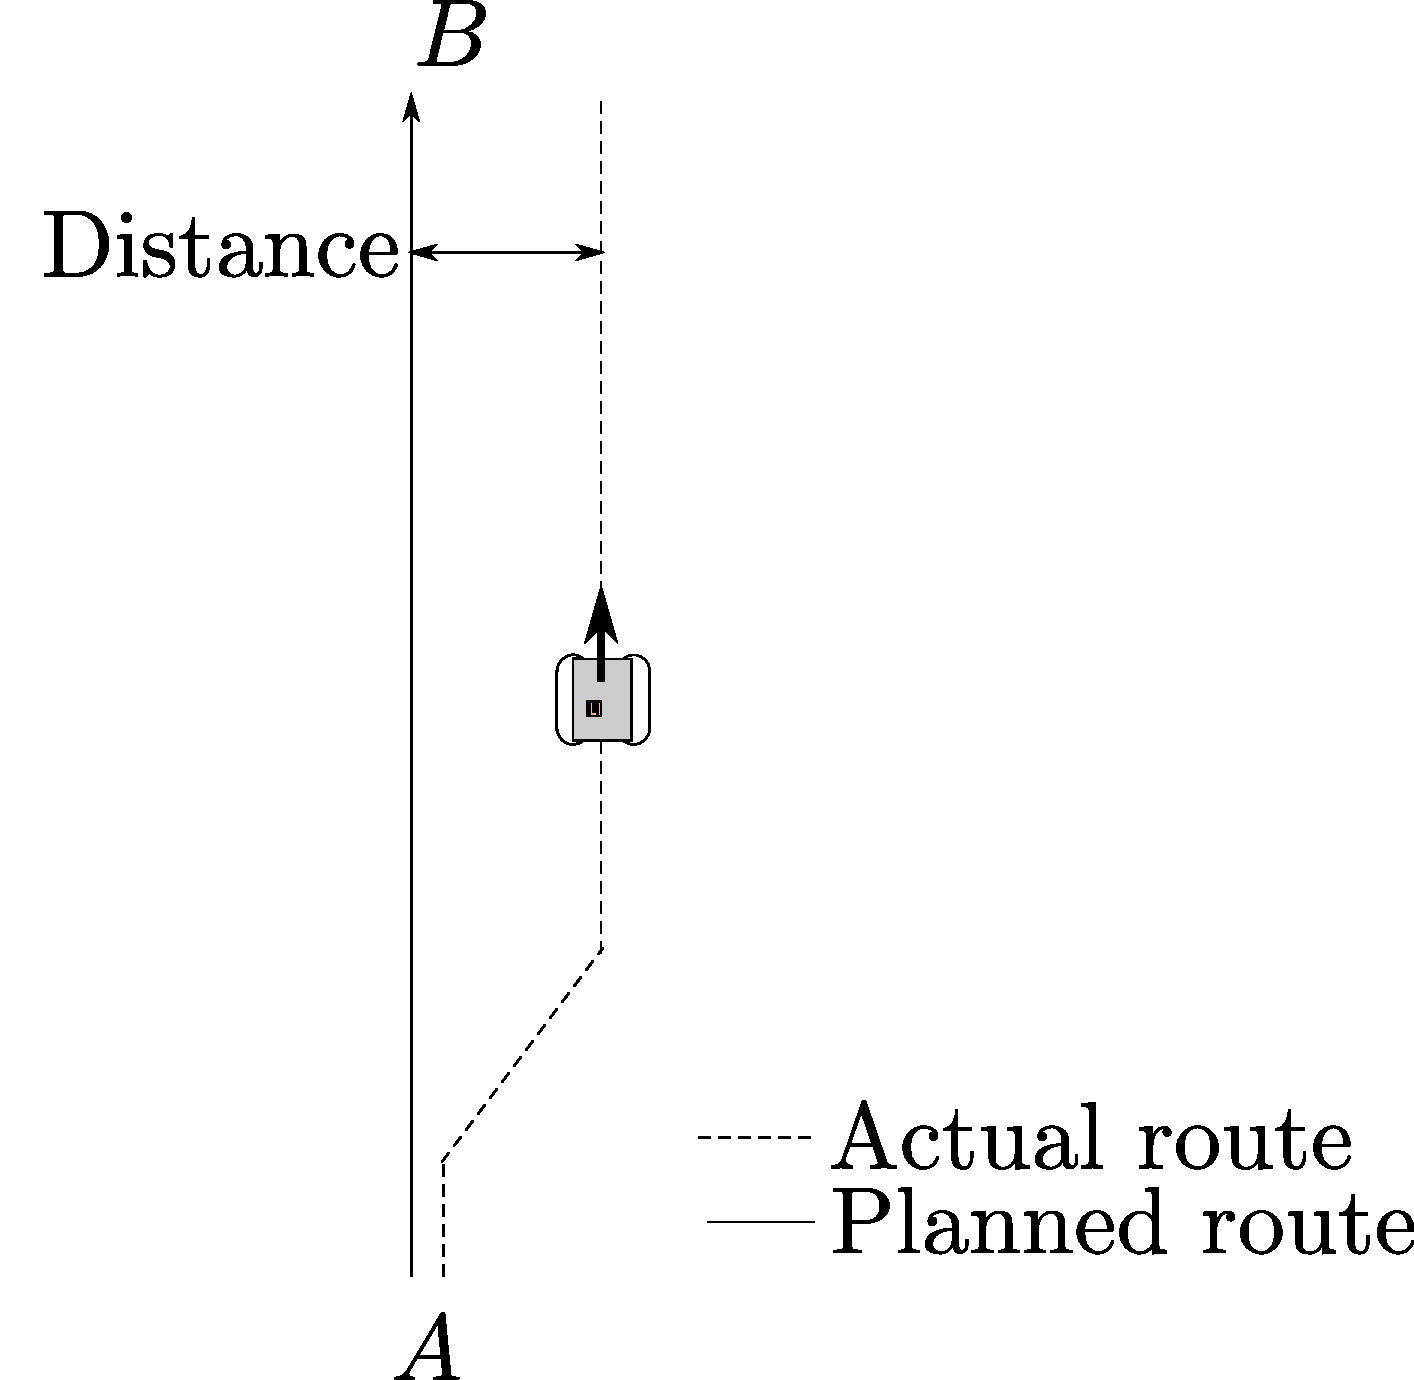
\includegraphics[scale=0.25]{Pictures/steeringDeviation.pdf}
      \end{figure}
    \end{minipage}
  \end{minipage}
\end{frame}

%- 5 -%
\begin{frame}{Parameter Estimation}{Fibonacci Line Search}
  \begin{minipage}{\linewidth}
    \begin{minipage}{0.40\linewidth}
      \only<1>{
      \begin{figure}[H]
        \centering
        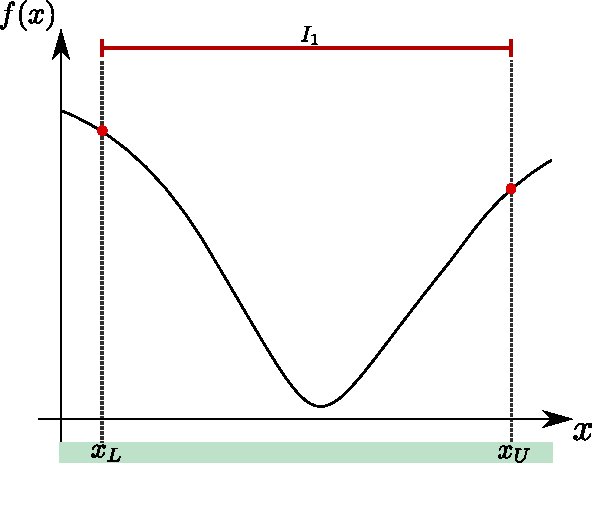
\includegraphics[scale=0.40]{Pictures/fibonacciIntervalSystem0}
      \end{figure}
      }
      \only<2>{
      \begin{figure}[H]
        \centering
        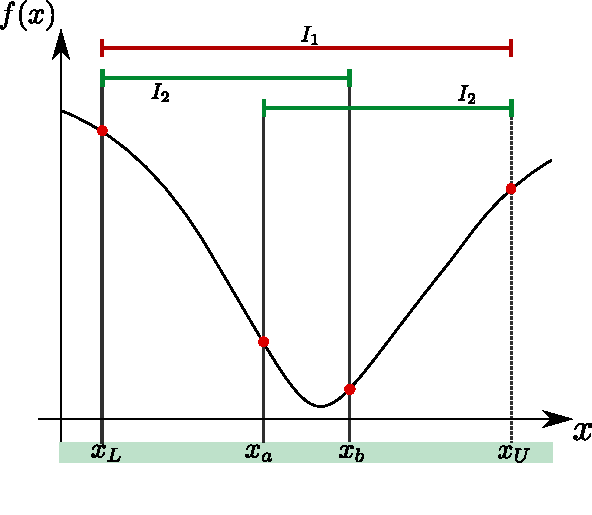
\includegraphics[scale=0.40]{Pictures/fibonacciIntervalSystem1}
      \end{figure}
      }
      \only<3>{
      \begin{figure}[H]
        \centering
        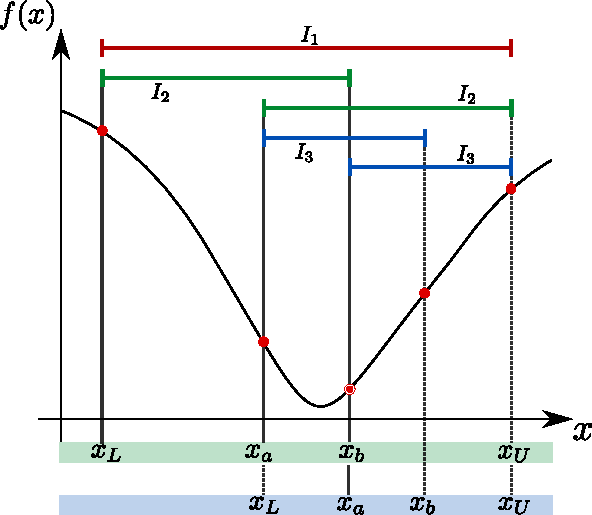
\includegraphics[scale=0.40]{Pictures/fibonacciIntervalSystem2}
      \end{figure}
      }
      \only<4->{
      \begin{figure}[H]
        \centering
        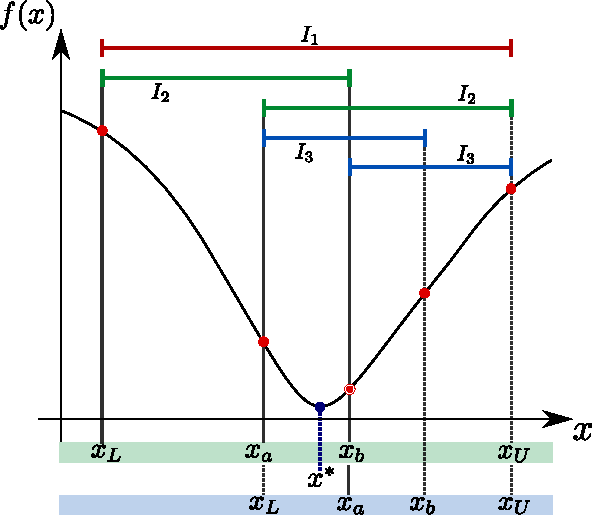
\includegraphics[scale=0.40]{Pictures/fibonacciIntervalSystem3}
      \end{figure}
      }
    \end{minipage}
    % \hspace{0.05\linewidth}
    \begin{minipage}{0.45\linewidth}
      \pause[5]
      % \only<5->{
        \begin{itemize}
          \item Initial relations
        \end{itemize}
        \begin{displaymath}
          \si{I_k = I_{k+1} + I_{k+2}, for\ all\ k=1,2,\dots,n-1}
        \end{displaymath}
        \begin{displaymath}
          \si{I_n = I_{n+1},\ assuming\ I_{n+2}=0}
        \end{displaymath}
      % }
      \vspace{-12pt}
      %%
      \pause[6]
      % \only<6>{  
        \begin{itemize}
          \item Successive relations
        \end{itemize}
        \begin{displaymath}
          \si{I_{n+1}}      =  \phantom{\si{\ I_{n+1}  + I_{n+2}         =}}\si{ 1 I_n  = F_0 I_n}
        \end{displaymath}
        \begin{displaymath}
          \si{I_{n}}\phantom{_{+1}}      =  \si{ I_{n+1}  + I_{n+2} }                    =  \si{ 1 I_n  = F_1 I_n }
        \end{displaymath}
        \begin{displaymath}
          \si{I_{n-1}}      =  \si{ I_{n} }\phantom{_{+1}} + \si{ I_{n+1} } =  \si{ 2 I_n  = F_2 I_n }
        \end{displaymath}
        \begin{displaymath}
          \vdots
          \phantom{I_{n-4}+I_{n-5}+I{4242}}
        \end{displaymath}
        \begin{displaymath}
          \si{I_{k}}\phantom{_{4}}   =  \si{ I_{k+1} + I_{k+2} = F_{n-k+1} I_n }
        \end{displaymath}
        \begin{displaymath}
          \vdots                         
          \phantom{I_{n-4}+I_{n-5}+I{4242}}
        \end{displaymath}
        \begin{displaymath}
          \si{I_{1}}\phantom{_{4}}      =  \si{ I_{2}  + I_{3} }\si{= F_n I_n }\phantom{_{k-1k+2k+3}} 
        \end{displaymath}
      % }
    \end{minipage}
  \end{minipage}
\end{frame}


%----------------------------------------------------------------
\begin{frame}{Parameter Estimation}{Forward-Backward Method}
  \begin{minipage}{\linewidth}
    \begin{minipage}{0.35\linewidth}
      \begin{figure}[H]
        \centering
        Figures showing a convex function with numbered high-low-high points
        % 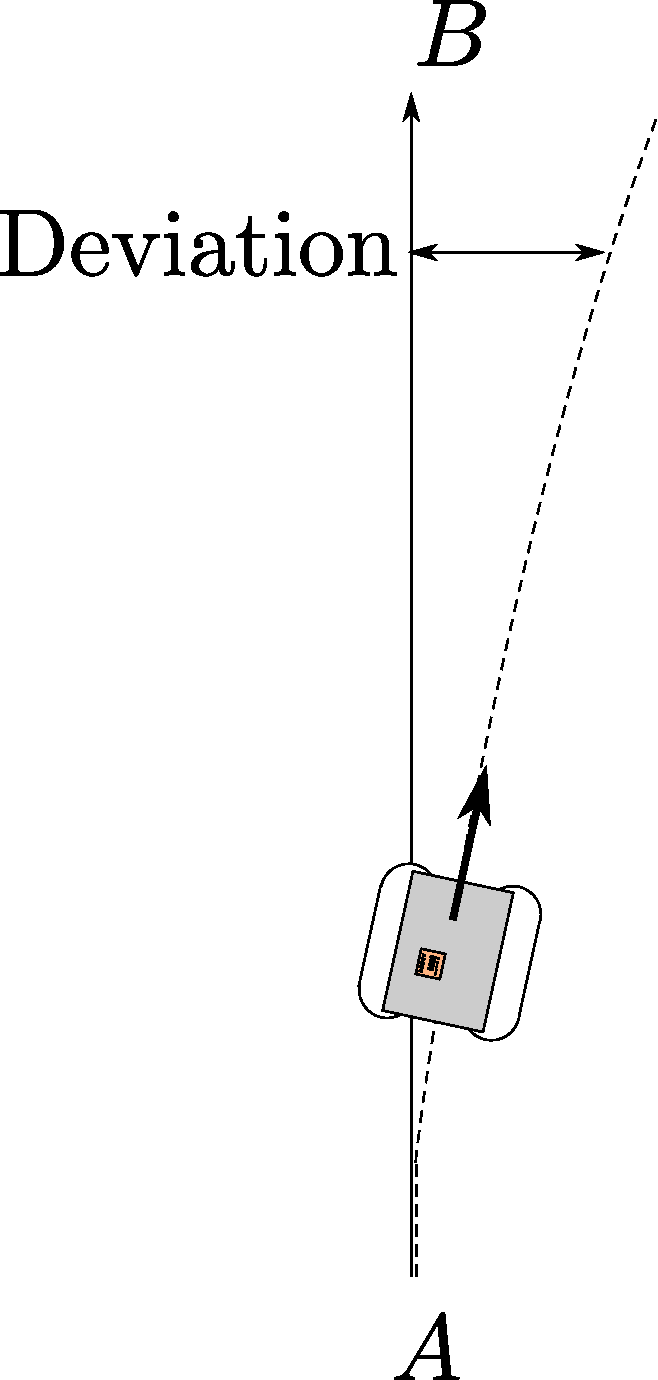
\includegraphics[scale=0.25]{Pictures/vehicleLineDeviation.pdf}
      \end{figure}
    \end{minipage}
    \hspace{0.03\linewidth}
    \begin{minipage}{0.45\linewidth}
      \begin{figure}[H]
        \centering
        Figures showing a convex function with numbered high-low-high points (2nd configuration)
        % 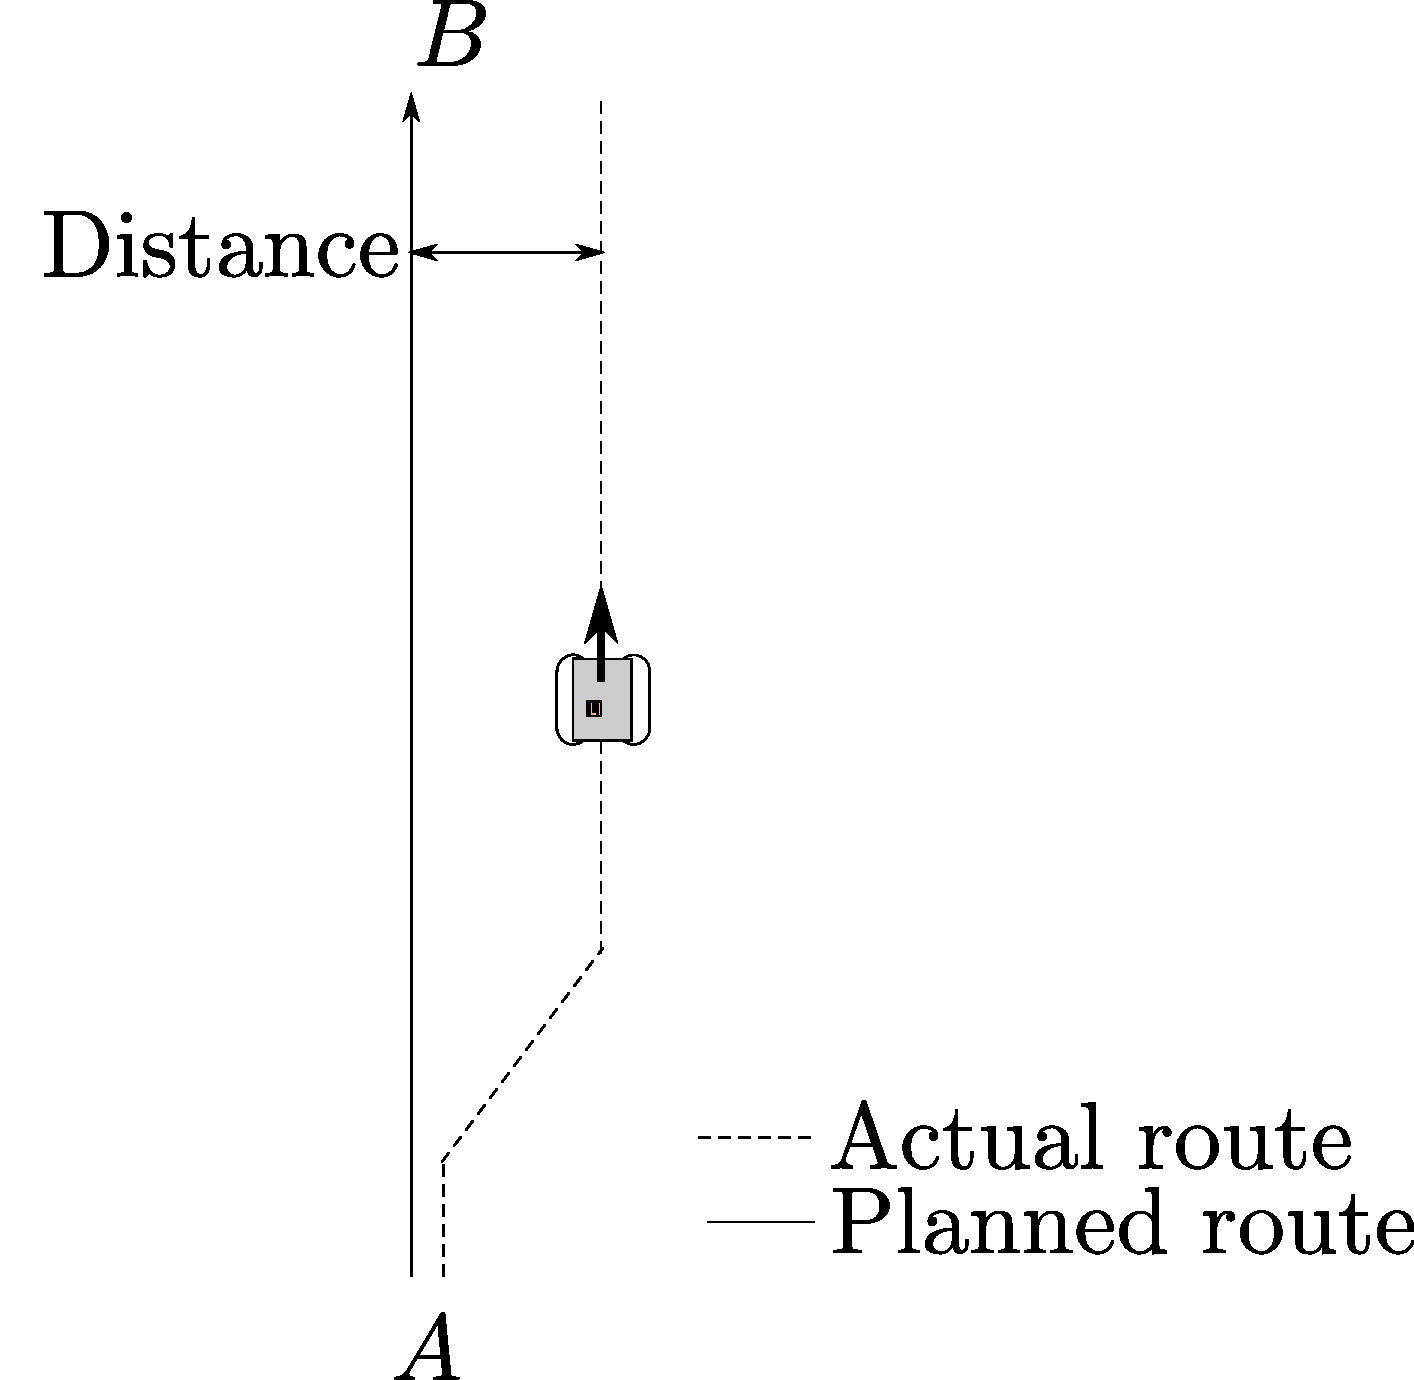
\includegraphics[scale=0.25]{Pictures/steeringDeviation.pdf}
      \end{figure}
    \end{minipage}
  \end{minipage}
\end{frame}

\begin{frame}{Parameter Estimation}{Implementation (1)}
  \begin{minipage}{\linewidth}\centering
    \begin{minipage}{0.35\linewidth}
      \begin{figure}[H]
        \centering
        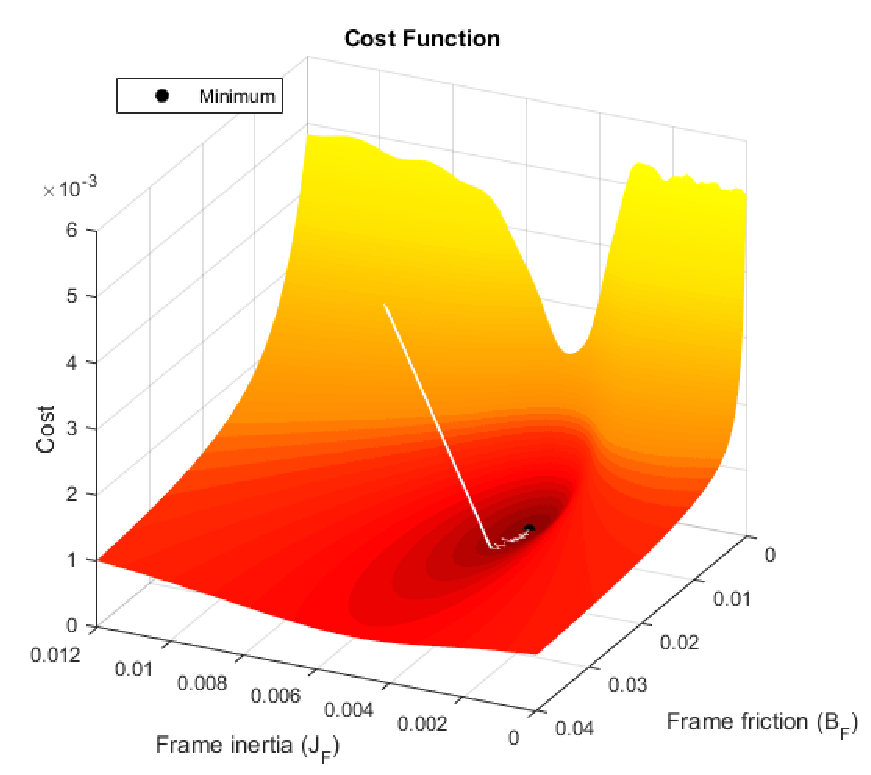
\includegraphics[scale=0.35]{Pictures/costFunctionMinimized.pdf}
      \end{figure}
    \end{minipage}
    \hspace{0.15\linewidth}
    \begin{minipage}{0.45\linewidth}
      \begin{figure}[H]
        \centering
        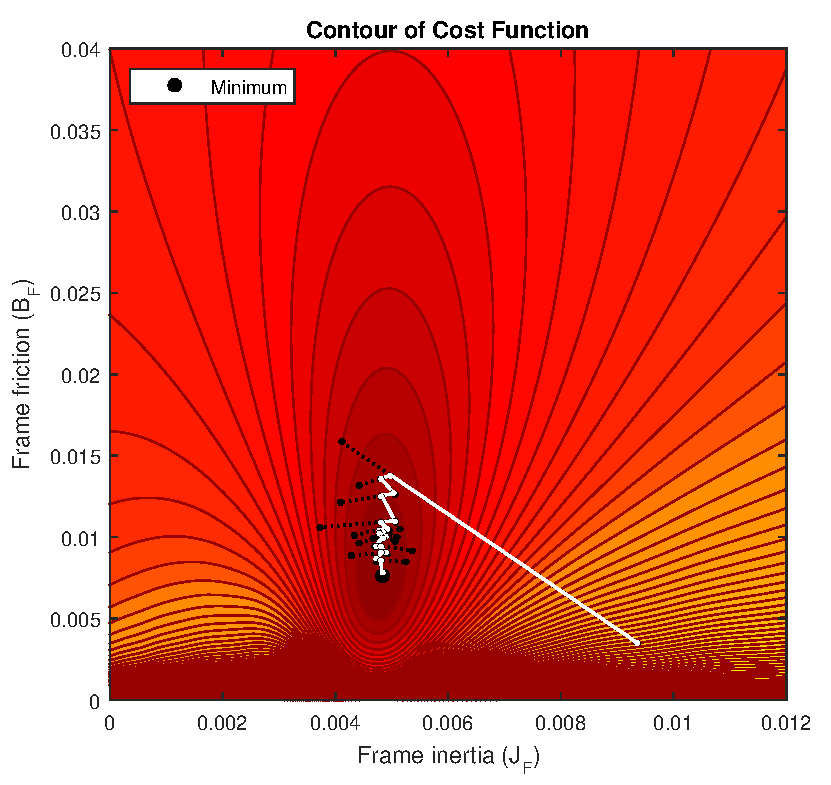
\includegraphics[scale=0.35]{Pictures/costFunctionMinimizedContour.pdf}
      \end{figure}
    \end{minipage}
  \end{minipage}
  Animated pictures would be better...
\end{frame}

\begin{frame}{Steering Model and Control}{Implementation (2)}
  \begin{minipage}{\linewidth}\centering
    \begin{minipage}{0.45\linewidth}
      \only<1->{
      \begin{figure}[H]
        \centering
        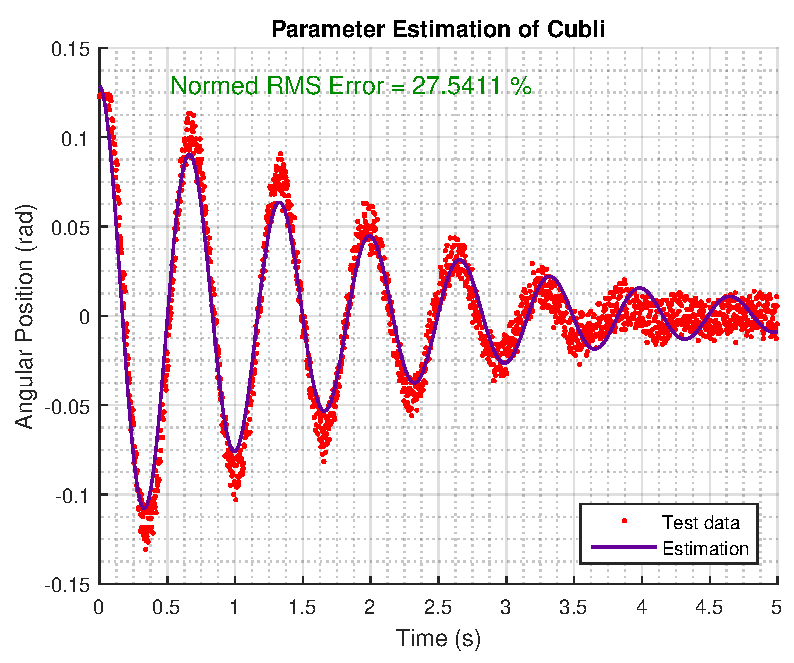
\includegraphics[scale=0.35]{Pictures/resultOfGradientWithFibonacciAndForwardBackward}
      \end{figure}
        \begin{table}[H]\centering
          \begin{tabular}{
          |c
          |S[table-figures-exponent=1,table-number-alignment=left, table-figures-integer=1]%@{\,}
          |s[table-unit-alignment = left,table-column-width=52pt]|}
            % \hline
              % \textbf{Parameter}  & \multicolumn{1}{c|}{\textbf{Value}} & \multicolumn{1}{c|}{\textbf{Unit}}\\
            \hline%------------------------------------------------------------------
              \si{J_F}            & 4.8e-3 & \kilo\gram\meter\squared         \\%& -\\
            % \hline%------------------------------------------------------------------
              \si{B_F}            & 7.8e-3 & \newton\metre\second\per\radian            \\%& -\\
            \hline%------------------------------------------------------------------
          \end{tabular}
        \end{table}
      }
    \end{minipage}
    \hspace{0.05\linewidth}
    \begin{minipage}{0.45\linewidth}
      % \only<2->{
      \pause[2]
        \begin{figure}[H]
          \centering
          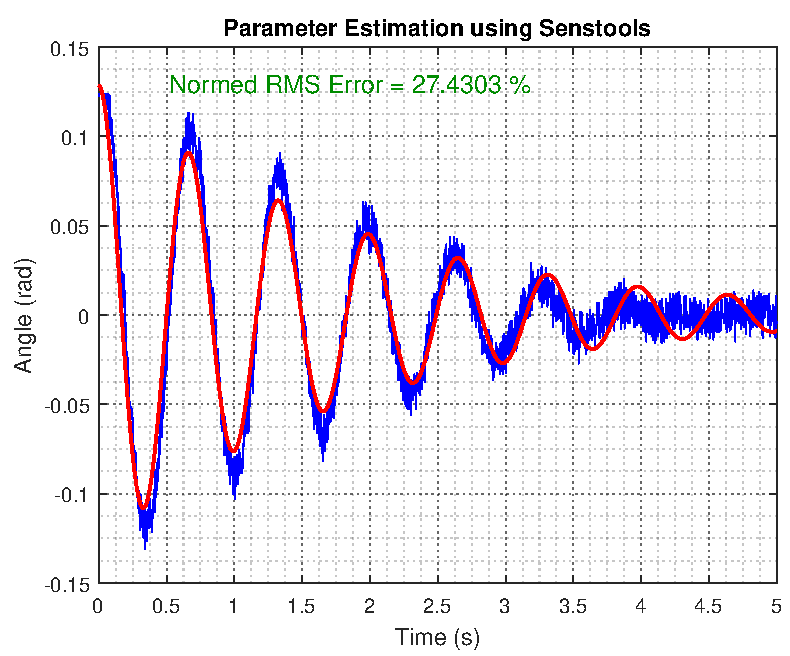
\includegraphics[scale=0.35]{Pictures/SenseToolParameterEstimation}
        \end{figure}
        \begin{table}[H]\centering
          \begin{tabular}{
          |c
          |S[table-figures-exponent=1,table-number-alignment=left, table-figures-integer=1]%@{\,}
          |s[table-unit-alignment = left,table-column-width=52pt]|}
            % \hline
              % \textbf{Parameter}  & \multicolumn{1}{c|}{\textbf{Value}} & \multicolumn{1}{c|}{\textbf{Unit}}\\
            \hline%------------------------------------------------------------------
              \si{J_F}            & 4.8e-3 & \kilo\gram\meter\squared             \\%& -\\
            % \hline%------------------------------------------------------------------
              \si{B_F}            & 7.7e-3 & \newton\metre\second\per\radian            \\%& -\\
            \hline%------------------------------------------------------------------
          \end{tabular}
        \end{table}
      % }
    \end{minipage}
  \end{minipage}
\end{frame}

%------------------------------------------------------------
\subsection{Model Parameters (rev'd)}

\begin{frame}{Model Parameters}{Final Parameters}
  \begin{table}[H]\centering
  \begin{tabular}{
  |c
  |S[
    table-figures-exponent=2,
    % table-column-width=60pt
    % table-figures-integer=2,
    % table-number-alignment=right
    ]
  |s[table-unit-alignment = left]|
  }
    \hline
      \textbf{Parameter}  & \multicolumn{1}{c|}{\textbf{Value}} & \multicolumn{1}{c|}{\textbf{Unit}}\\
    \hline%------------------------------------------------------------------
      \si{m_W}            & 0.222                               & \kilo\gram\\
    % \hline%------------------------------------------------------------------
      \si{l_W}            & 0.093                               & \metre\\
    % \hline%------------------------------------------------------------------
      \si{J_W}            & 0.601e-3                            & \kilo\gram\meter\squared\\
    % \hline%------------------------------------------------------------------
      \si{B_W}            & 17.03e-6                            & \newton\metre\second\per\radian\\
    % \hline%------------------------------------------------------------------
      \si{m_F}            & 0.548                               & \kilo\gram\\
    % \hline%------------------------------------------------------------------
      \si{l_F}            & 0.08498                             & \metre\\
    % \hline%------------------------------------------------------------------
      \si{J_F}            & 4.8e-3                              & \kilo\gram\meter\squared \\
    % \hline%------------------------------------------------------------------
      \si{B_F}            & 7.7e-3                              & \newton\metre\second\per\radian\\
    \hline%------------------------------------------------------------------
  \end{tabular}
  \end{table}
\end{frame}
%-----------------------------------------------------------------
\subsection{Model Testing}
\begin{frame}{Model Testing}{Linearization of the Model}
  \begin{itemize}
    \item Plant transfer function
  \end{itemize}
  \begin{displaymath}
    \si{G(s) = \frac{-148,8 \cdot s}{s^3 + 1,177 \cdot s^2 - 98,19 \cdot s - 2,783}}
  \end{displaymath}
  \pause
  \begin{itemize}
    \item Linear approximation
  \end{itemize}
  \begin{minipage}{\linewidth}\centering
    \begin{minipage}{0.45\linewidth}
      \begin{figure}[H]
        \centering
        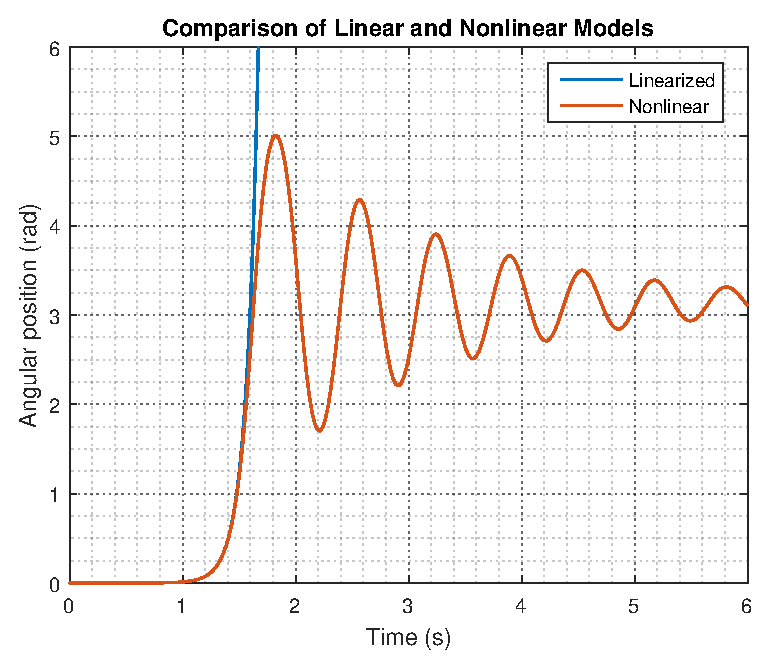
\includegraphics[scale=0.33]{Pictures/LinearizedVSNonlinear}
      \end{figure}
    \end{minipage}
    % \hspace{0.05\linewidth}
    \begin{minipage}{0.45\linewidth}
      \begin{figure}[H]
        \centering
        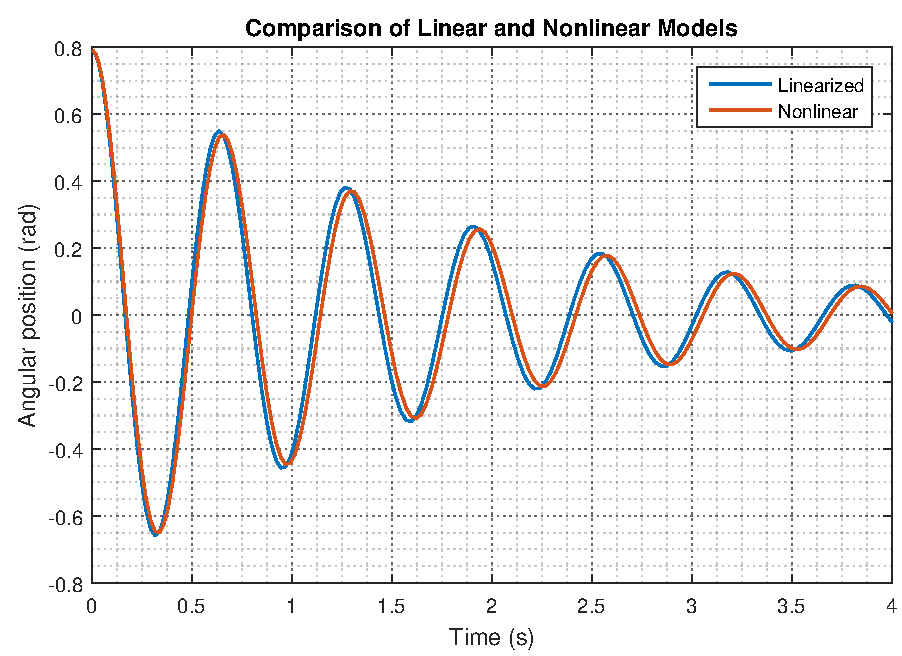
\includegraphics[scale=0.33]{Pictures/LinearizedVSNonlinear_0}
      \end{figure}
    \end{minipage}
  \end{minipage}
\end{frame}

\begin{frame}{Model Testing}{Comparison with Real System}
  \begin{itemize}
    \item Fall tests
  \end{itemize}
  \begin{minipage}{\linewidth}\centering
    \begin{minipage}{0.45\linewidth}
      \begin{figure}[H]
        \centering
        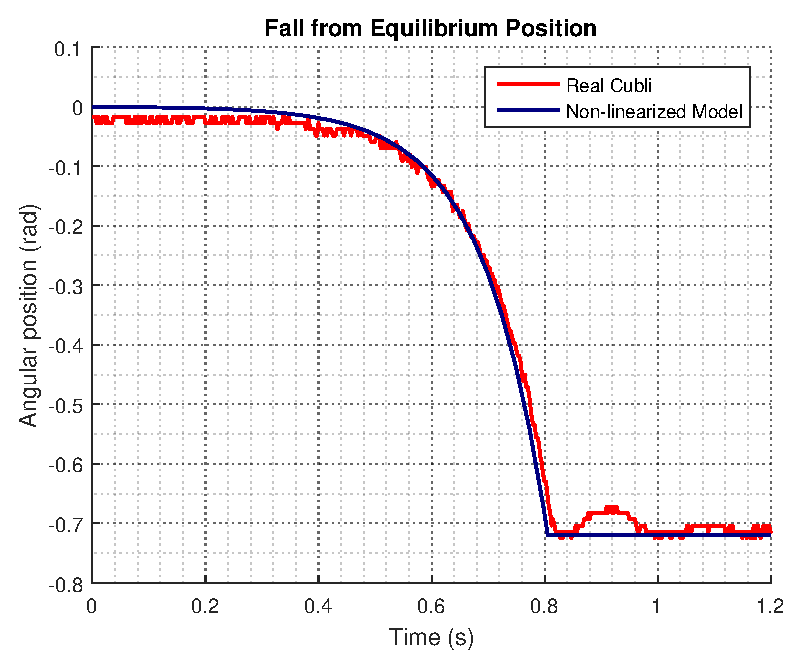
\includegraphics[scale=0.33]{Pictures/FallTestComparison}
      \end{figure}
    \end{minipage}
    % \hspace{0.05\linewidth}
    \begin{minipage}{0.45\linewidth}
      \begin{figure}[H]
        \centering
        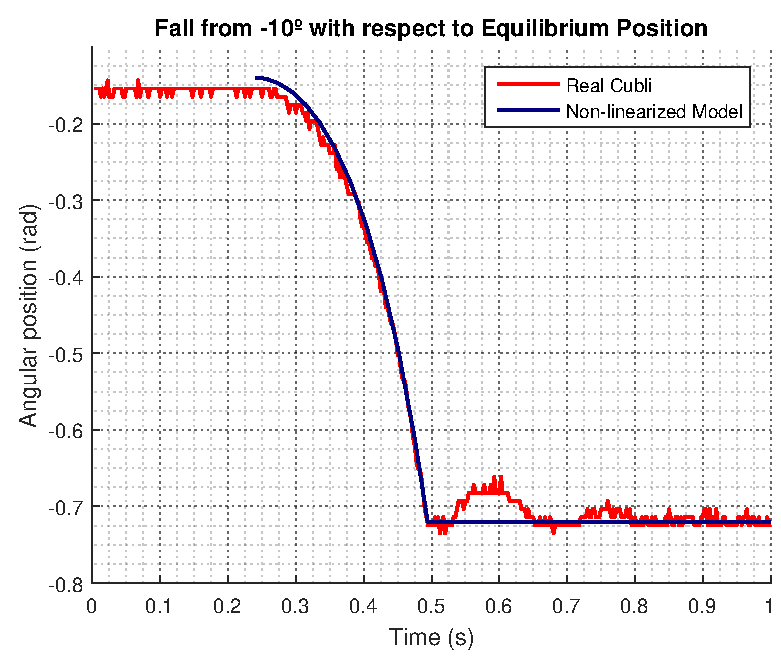
\includegraphics[scale=0.33]{Pictures/FallTestComparison10deg}
      \end{figure}
    \end{minipage}
  \end{minipage}
\end{frame}